\documentclass[11pt]{article}
\usepackage[margin=1in]{geometry}
\usepackage{amsmath,amssymb,amsthm}
\usepackage{booktabs}
\usepackage{graphicx}
\usepackage{hyperref}
\usepackage{xcolor}
\usepackage{microtype}
\hypersetup{
  pdftitle={Adinkra-Stabilized Hypercube Model: Canonical Algebra, Mapping Semantics, and Controlled Simulations},
  pdfauthor={James Daley},
  pdfsubject={Canonical finite mathematics and deterministic reference implementation for the ASH Model},
  pdfkeywords={binary linear code, hypercube, Adinkra, Garden algebra, deterministic reconstruction}
}

\newtheorem{theorem}{Theorem}
\newtheorem{proposition}{Proposition}
\newtheorem{definition}{Definition}

\title{Adinkra-Stabilized Hypercube Model:\\Canonical Algebra, Mapping Semantics, and Controlled Simulations}
\author{James Daley}
\date{Version 1.1.0 -- June 2026}

\begin{document}
\maketitle

\begin{abstract}
The Adinkra-Stabilized Hypercube (ASH) Model is an exploratory finite-state framework on $\mathbb F_2^9$.  This paper gives a canonical, executable construction: a rank-four doubly-even linear $[9,4,4]$ transform code; a parity-valid application-state subspace; strict one-bit bounded-distance recovery; an idempotent code-orbit projection; and an $N=8$ Adinkra/Garden representation obtained from the punctured self-dual $[8,4,4]$ code.  It also specifies eight deterministic image/video measurements, coordinate-9 parity, temporal hysteresis, bounded branch semantics, reconstruction operators, source-consistency scoring, and pruning.  Controlled simulations show that the bell-shaped Hamming-weight histogram is the $\operatorname{Binomial}(9,1/2)$ marginal of uniform occupancy and is not evidence uniquely caused by ASH transforms.  Proven finite mathematics, deterministic computation, and interpretive procedural cosmology are therefore stated separately.
\end{abstract}

\section{Scope}
ASH studies the composition of finite binary states, code symmetries, graph quotients, procedural branching, and reproducible media-processing semantics.  The present contribution is a rigorous finite model and reference implementation.  It is not an empirical confirmation of a cosmological theory.

Earlier versions used a genuine coding-theory scaffold but described it imprecisely: a length-nine code was called self-dual, simulations without a decoder were described as correcting errors, and a generic random-state histogram was presented as ASH-specific convergence.  Version 1.1.0 resolves those discrepancies.

\section{Nine-bit state space}
Let
\[
V=\mathbb F_2^9.
\]
Its $2^9=512$ states are the vertices of the hypercube $Q_9$.  Two states are adjacent when their Hamming distance is one, so each vertex has degree nine.  Plane $k$ consists of states of weight $k$ and contains $\binom{9}{k}$ vertices.

Application mapping uses
\[
E=\{x\in V:x_9=x_1\oplus\cdots\oplus x_8\}.
\]
This is the kernel of nonzero total parity, hence $\dim E=8$ and $|E|=256$.

\begin{figure}[ht]
\centering
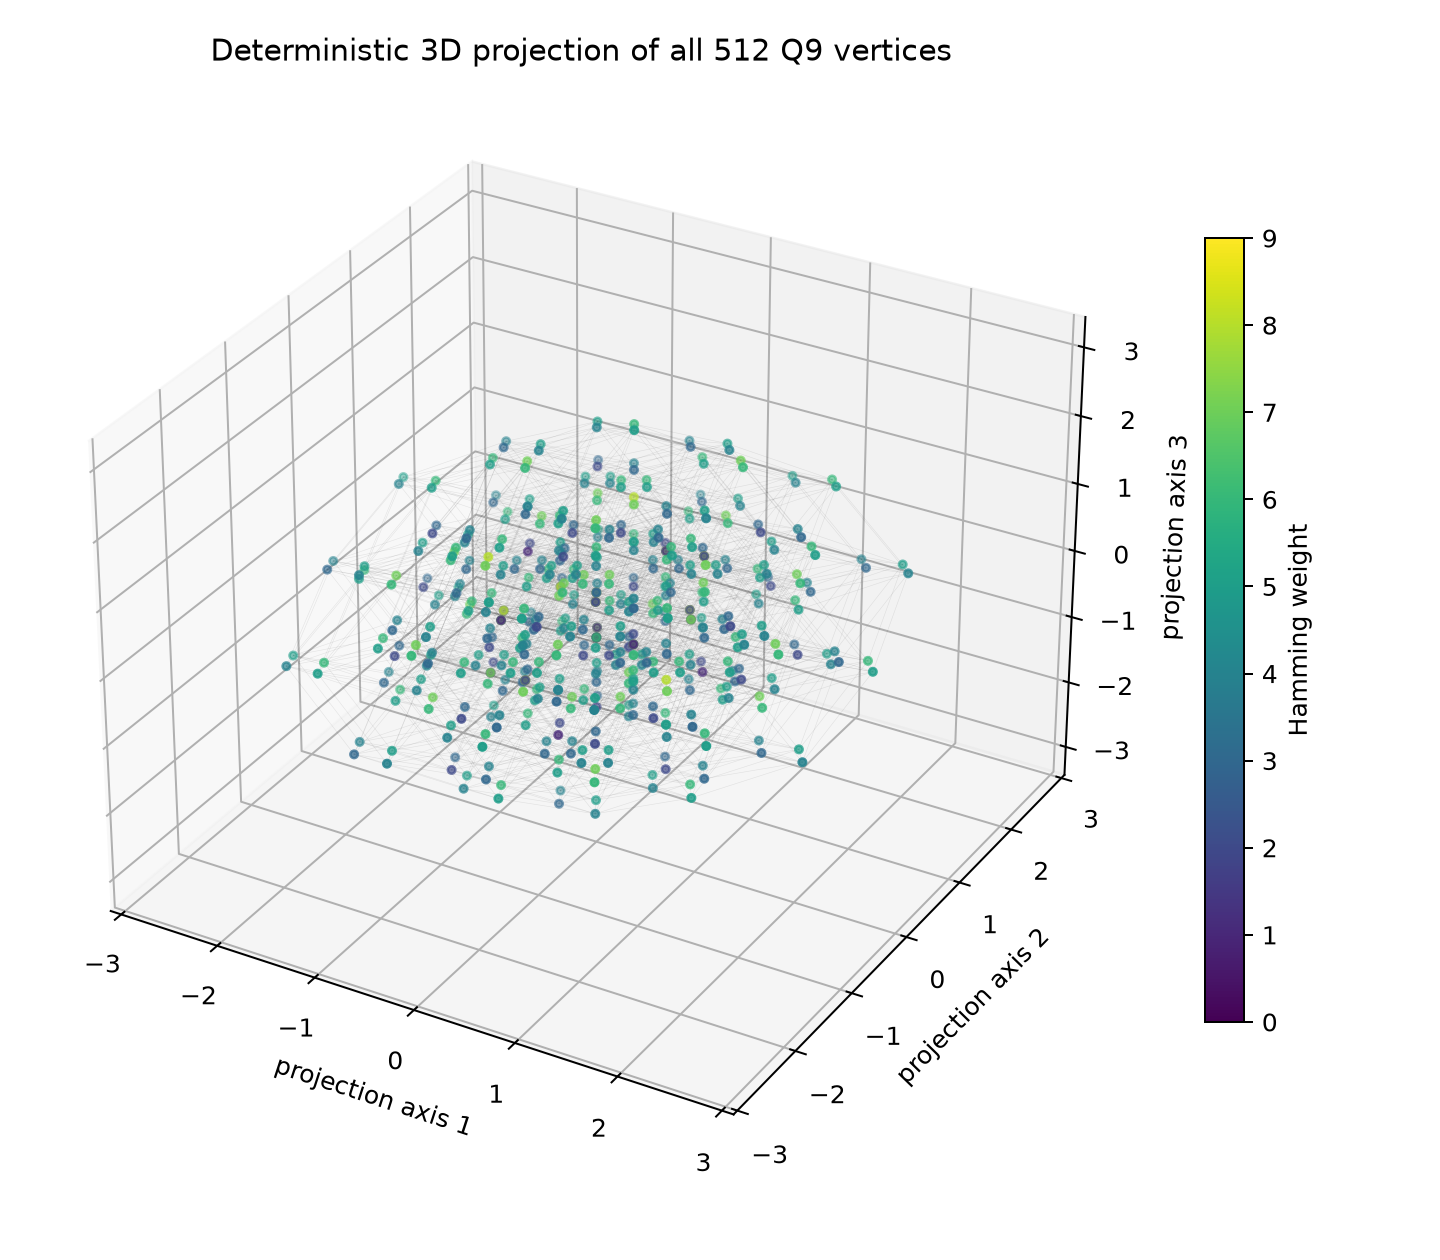
\includegraphics[width=0.82\textwidth]{../figures/hypercube-3d-projection.png}
\caption{Documented linear visualization of all 512 vertices and all 2,304 edges.  It is illustrative, not a physical embedding.}
\end{figure}

\section{Canonical transform code}
The code $C$ is the row span over $\mathbb F_2$ of
\[
G=\begin{pmatrix}
1&1&1&1&0&0&0&0&0\\
1&1&0&0&1&1&0&0&0\\
1&0&1&0&1&0&1&0&0\\
1&0&0&1&1&0&0&0&1
\end{pmatrix}.
\]
Row reduction has four pivots, so $\dim C=4$ and $|C|=16$.  Exhaustive encoding gives the weight distribution
\[
A_0=1,\qquad A_4=14,\qquad A_8=1.
\]
Thus $C$ is doubly even, and its minimum nonzero weight is four.  Since the code is linear,
\[
d_{\min}(C)=4.
\]

Column 8 of $G$ is zero, so $c_8=0$ for every $c\in C$.  Each generator satisfies
\[
c_9=c_1\oplus\cdots\oplus c_8,
\]
and linearity extends this relation to the entire code.  Coordinate 9 is active because the fourth generator has $c_9=1$.

\begin{proposition}
$C$ is self-orthogonal but is not self-dual in $\mathbb F_2^9$.
\end{proposition}
\begin{proof}
For $u,v\in C$,
\[
\operatorname{wt}(u+v)=\operatorname{wt}(u)+\operatorname{wt}(v)-2|\operatorname{supp}(u)\cap\operatorname{supp}(v)|.
\]
All three weights are divisible by four, so the intersection size is even and $u\cdot v=0$.  Hence $C\subseteq C^\perp$.  But $\dim C=4$ and $\dim C^\perp=9-4=5$, so equality is impossible.
\end{proof}

Puncturing coordinate 8 is injective and gives a doubly-even $[8,4,4]$ code $C_8$.  It is self-orthogonal and has half the ambient dimension, so it is self-dual.

\section{Strict error recovery}
A four-bit message $m$ is encoded as $mG$.  Decoding computes distance to all 16 codewords and succeeds only at distance zero or one.

\begin{theorem}
Every one-bit corruption of a codeword is uniquely corrected.
\end{theorem}
\begin{proof}
Let $d(r,c)\leq1$.  For any other codeword $c'$, the triangle inequality gives
\[
d(r,c')\geq d(c,c')-d(r,c)\geq4-1=3.
\]
Thus $c$ is the unique nearest codeword.
\end{proof}

The 16 radius-one balls are disjoint and each contains $1+9=10$ states.  The exhaustive decoder partition is 16 exact states, 144 corrected states, and 352 rejected states.  All $16\binom92=576$ two-bit corruptions are rejected; a unique nearest codeword at distance two is not accepted.

For a known affine anchor $a$, a valid branch state is $a+c$.  Decoding $(r+a)$ recovers $c$ through one bit, then reconstructs $a+c$.  The implementation checks all 256 integrity-valid anchors, all 16 codewords, and all nine one-bit errors, for 36,864 affine corrections.

\begin{figure}[ht]
\centering
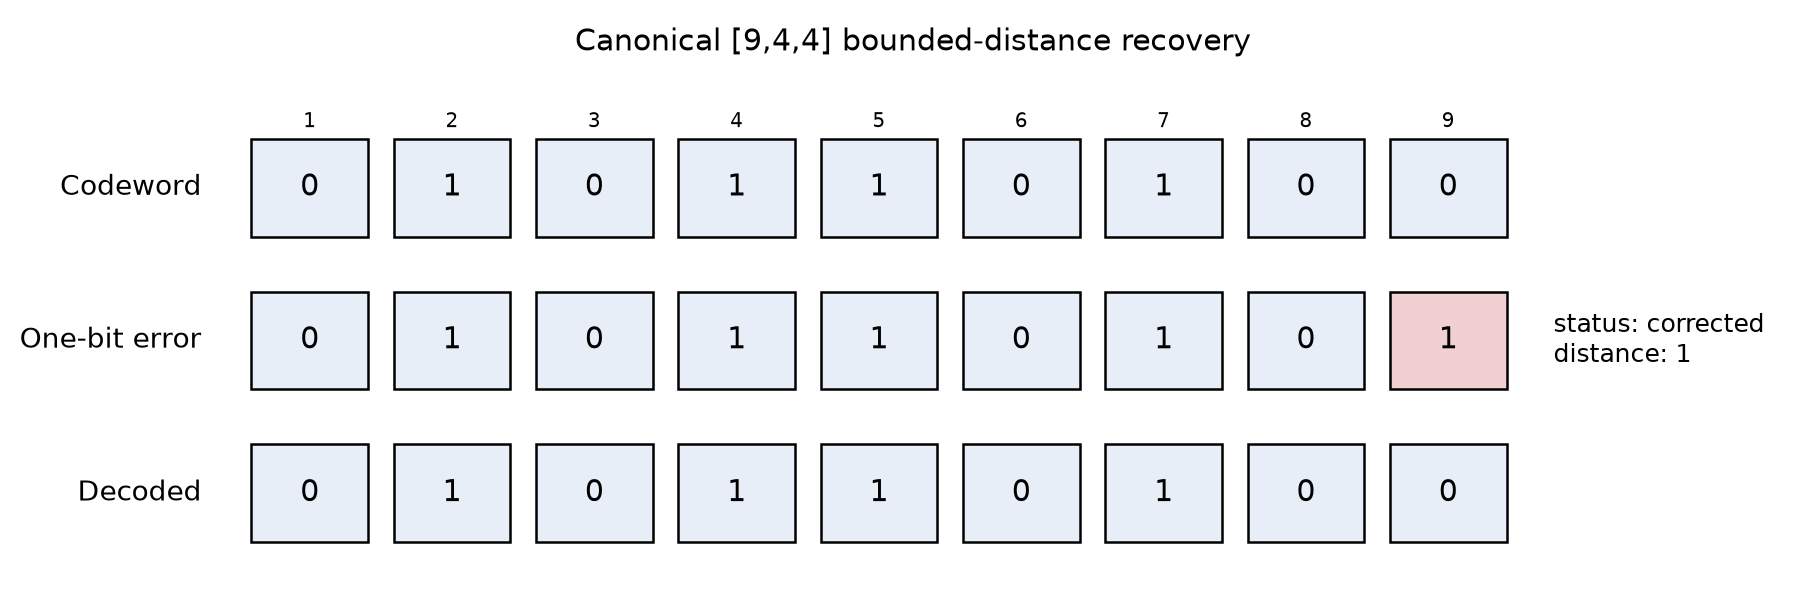
\includegraphics[width=0.94\textwidth]{../figures/single-bit-error.png}
\caption{Generated nine-bit one-error example and bounded-distance recovery.}
\end{figure}

\section{Code orbits and projection}
The additive action of $C$ partitions $V$ into 32 orbits of size 16, and $E$ into 16 such orbits.  Coordinate 8 is constant on every orbit.

For $f:V\to\mathbb R$, define
\[
(Tf)(x)=\frac1{|C|}\sum_{c\in C}f(x+c).
\]
Then
\[
(T^2f)(x)=\frac1{|C|^2}\sum_{a,b\in C}f(x+a+b).
\]
For every fixed $d\in C$, exactly $|C|$ pairs satisfy $a+b=d$.  Therefore $T^2=T$.  Reindexing also shows that $T$ is self-adjoint and that its image is exactly the space of functions constant on code orbits.  Random movement by one codeword is not the same operation as evaluating $T$; the implementation exposes exact and Monte Carlo averaging separately.

\section{Adinkra quotient and Garden algebra}
The quotient $Q_8/C_8$ has $2^8/2^4=16$ vertices.  Codeword parity is even, so parity is well-defined on cosets, producing eight bosonic and eight fermionic vertices.  Each vertex has one edge of each of eight colors, hence 64 undirected colored edges.

Let
\[
I=\begin{pmatrix}1&0\\0&1\end{pmatrix},\quad
X=\begin{pmatrix}0&1\\1&0\end{pmatrix},\quad
Z=\begin{pmatrix}1&0\\0&-1\end{pmatrix},\quad
J=\begin{pmatrix}0&1\\-1&0\end{pmatrix}.
\]
Define
\begin{align*}
L_1&=I\otimes I\otimes I,&L_2&=I\otimes I\otimes J,\\
L_3&=I\otimes J\otimes X,&L_4&=X\otimes J\otimes Z,\\
L_5&=Z\otimes J\otimes Z,&L_6&=J\otimes Z\otimes X,\\
L_7&=J\otimes I\otimes Z,&L_8&=J\otimes X\otimes X.
\end{align*}
These are signed permutation matrices and, with $R_I=L_I^T$, satisfy exactly
\[
L_IR_J+L_JR_I=2\delta_{IJ}I_8.
\]
The executable proof evaluates all 64 matrix pairs with integer residual zero and derives a color-preserving isomorphism with $Q_8/C_8$ after color permutation $(1,2,3,5,4,8,6,7)$.

\begin{figure}[ht]
\centering
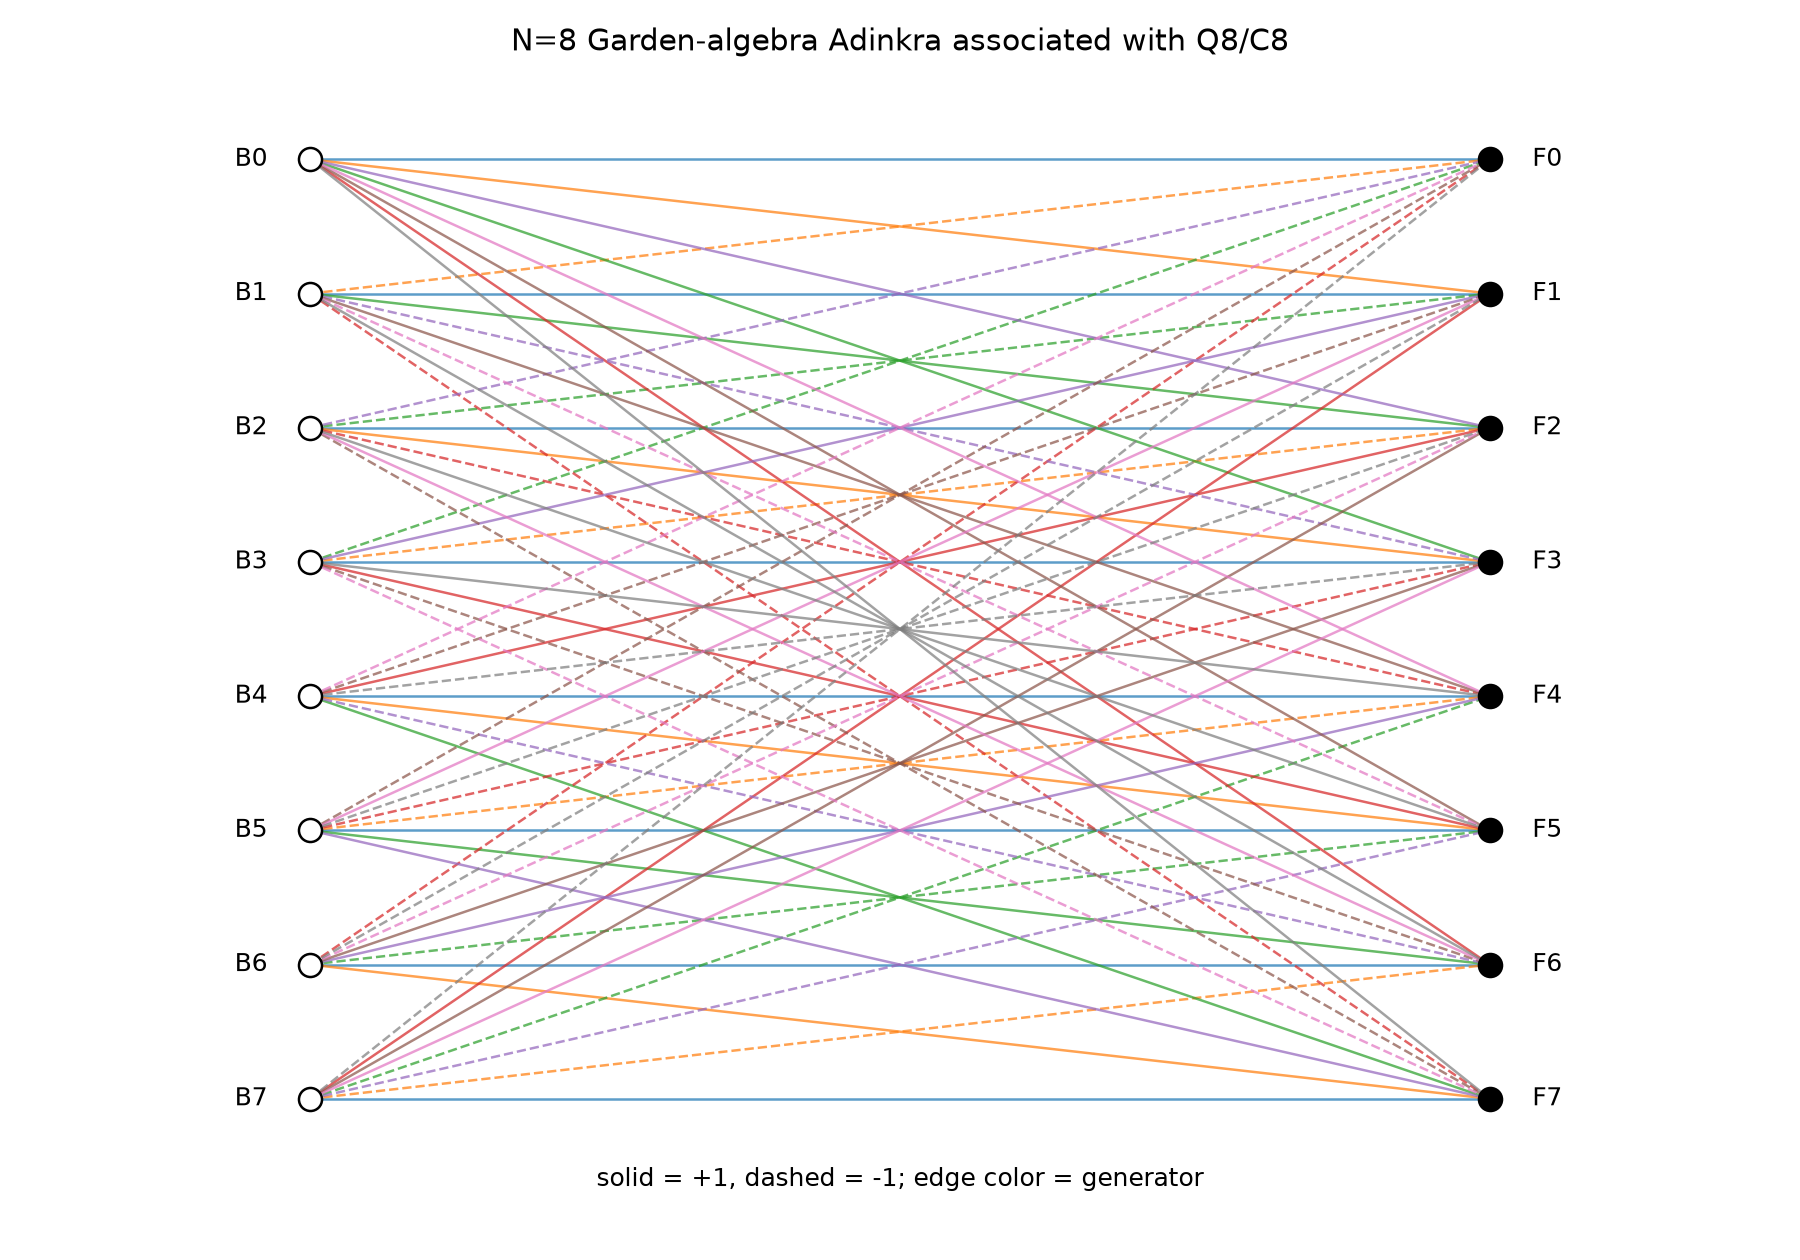
\includegraphics[width=0.9\textwidth]{../figures/adinkra-graph-colored.png}
\caption{Executable $N=8$ Garden representation.  Dashed edges denote negative entries.}
\end{figure}

\section{Image and video state mapping}
Eight measurements define coordinates 1--8: mean luminance, RMS contrast, edge energy, texture residual energy, chroma energy, horizontal-gradient energy, vertical-gradient energy, and temporal change.  Every measurement is normalized to $[0,1]$.  Fixed thresholds and hysteresis are normative in \texttt{config/ash\_mapping\_v1.json}.  Coordinate 9 is recomputed as parity.

Without history, ties at a threshold map to one.  With history, a zero bit switches on at threshold plus hysteresis and a one bit switches off below threshold minus hysteresis.  This defines a deterministic temporal transition and rejects an invalid prior state.

\section{Branch and reconstruction semantics}
Each semantic node has actions $0,+,-$ with weights $0.5,0.25,0.25$.  At level $\ell$, $+$ toggles message bit $\ell\bmod4$, $-$ toggles bit $(\ell+1)\bmod4$, and $0$ leaves the message unchanged.  A message is encoded to $c\in C$ and the branch state is $x+c$.

A depth-$d$ tree has $3^d$ leaves and $(3^{d+1}-1)/2$ total nodes.  Child probabilities sum to the parent probability, so total leaf weight is one.  Depth four has 81 leaves, 121 nodes, and reaches all 16 operator messages.

\begin{figure}[ht]
\centering
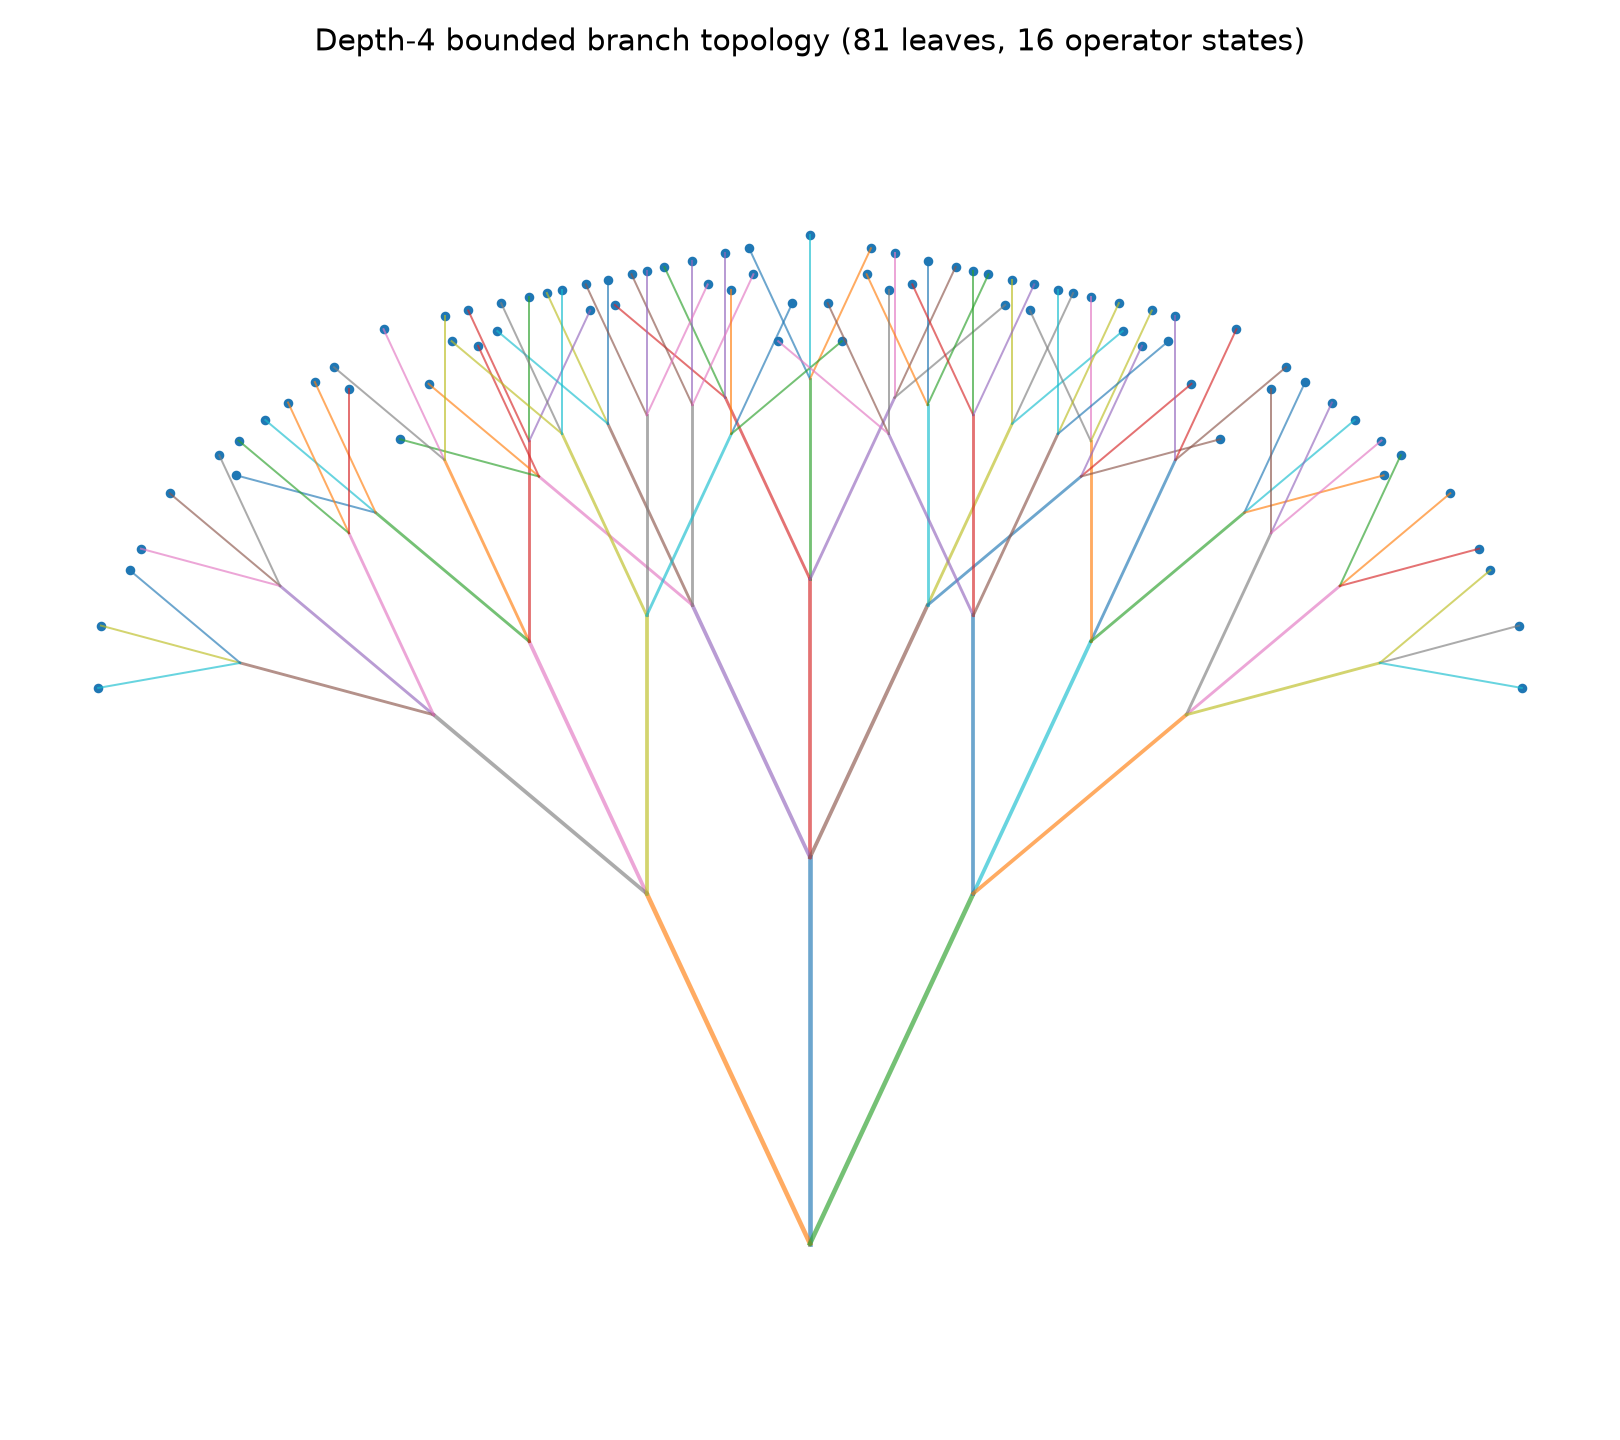
\includegraphics[width=0.78\textwidth]{../figures/branch-topology.png}
\caption{Depth-four bounded branch geometry: 81 leaves and 16 unique operator messages.}
\end{figure}

The reference operator family combines horizontal, vertical, and isotropic detail injection with isotropic regularization.  Candidates are clipped to $[0,1]$, reprojected to source resolution, scored by source, edge, and optional temporal loss, and deterministically pruned.  This is a conformance reference, not an image-quality claim.

\section{Controlled Markov dynamics}
For $0<p<1$, the noise kernel is
\[
P=(1-p)I+\frac p9\sum_{i=1}^{9}F_i,
\]
where $F_i$ flips coordinate $i$.  The chain is irreducible because bit flips generate $V$, aperiodic because $1-p>0$, and doubly stochastic because each $F_i$ is a permutation matrix.  Hence the unique stationary distribution is uniform.

Under uniform occupancy, Hamming weight is exactly
\[
\Pr(W=k)=\binom9k2^{-9}.
\]
Codeword translations are also permutations and preserve uniformity.  Thus a bell-shaped Hamming histogram is a uniform-state baseline, not ASH-specific evidence.

\begin{figure}[ht]
\centering
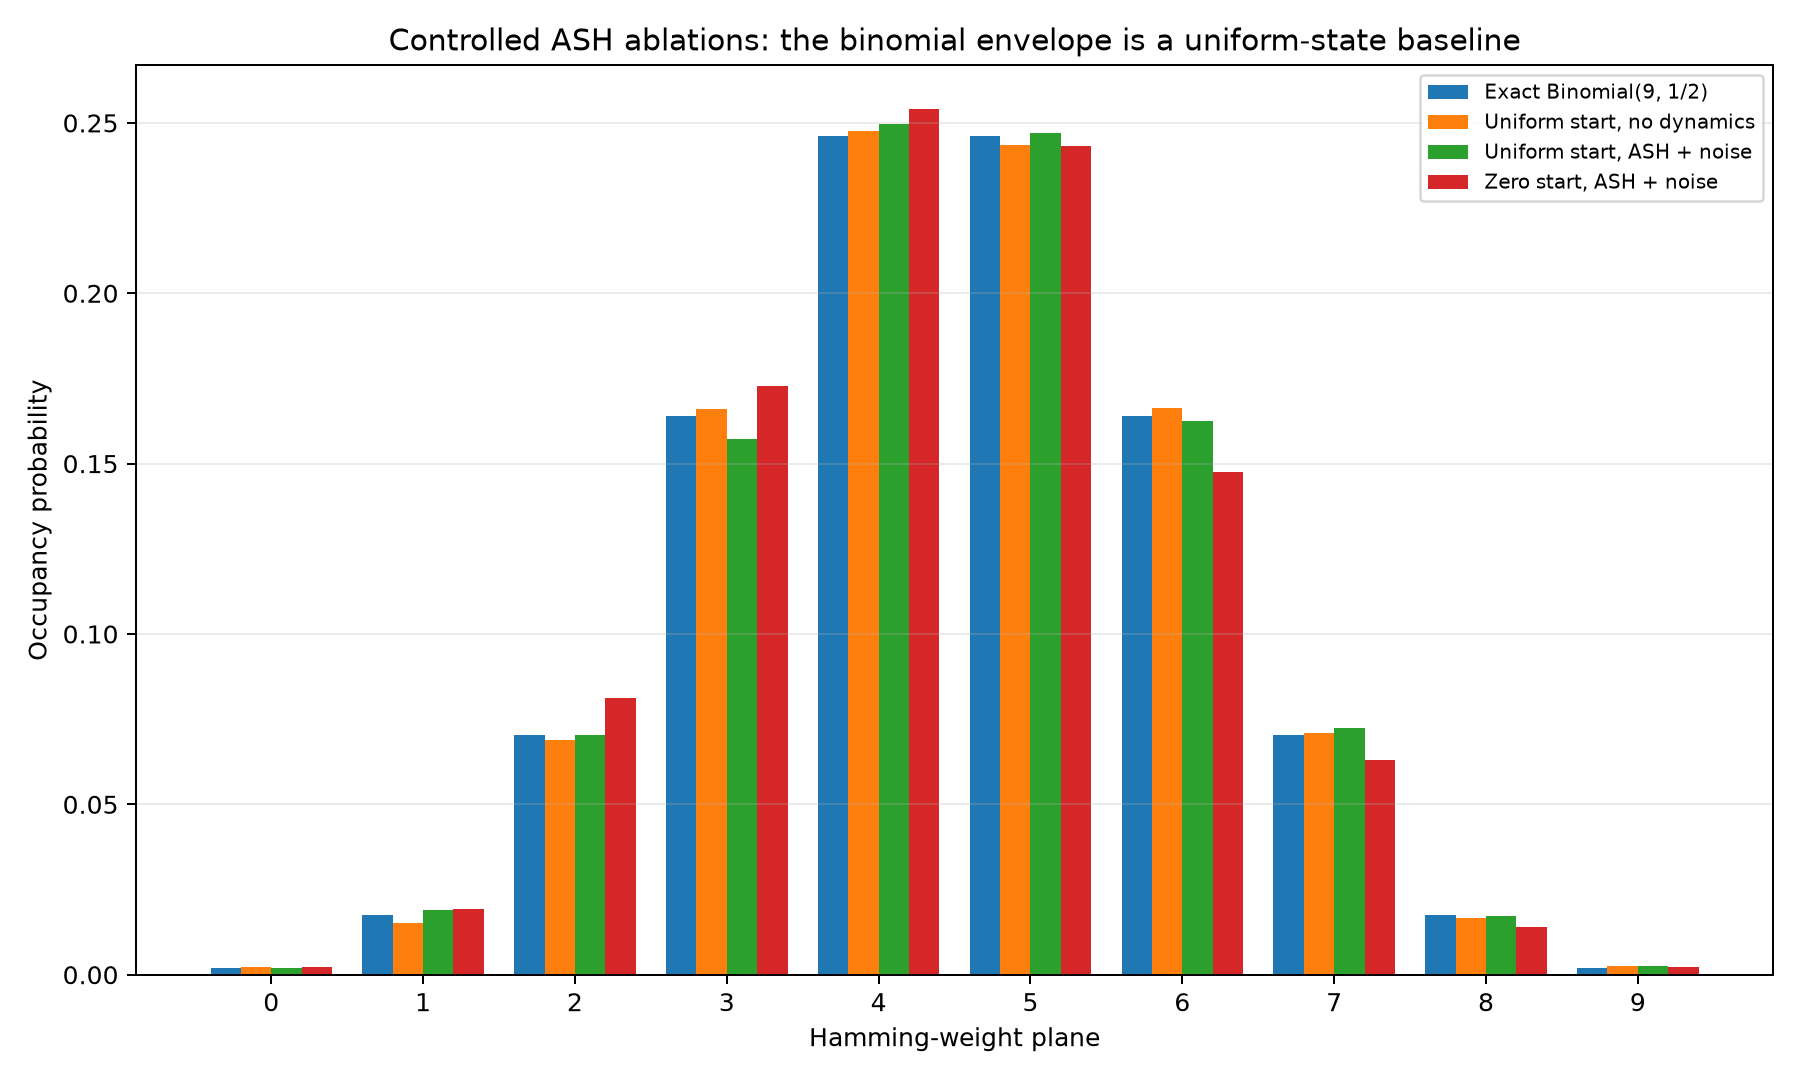
\includegraphics[width=0.96\textwidth]{../figures/simulation-histogram.png}
\caption{Controlled ablations against the exact binomial envelope.}
\end{figure}

Without noise, agents starting at zero and translated only by codewords remain in the 16-state code orbit and have weight support $\{0,4,8\}$ rather than a full binomial distribution.

\section{Verification and limitations}
The repository includes exhaustive tests across all 512 states, all one- and two-bit codeword neighborhoods, all parity-valid affine anchors, exact Garden identities, a quotient-graph isomorphism, state and codeword tables, branch topology, controlled ablations, and source/artifact hashes.

The implementation establishes the finite mathematics and deterministic semantics described here.  The feature thresholds, branch priors, geometry constants, reconstruction operators, and score weights are versioned reference-design choices; they are not uniquely derived from the interpretive axioms or empirically calibrated as optimal.  The implementation does not establish empirical cosmology, a derivation of quantum measurement probabilities, ASH-specific Gaussian causation, observed physical supersymmetry, or superior image quality.  Those claims require separately designed evidence and matched controls.

\section{Conclusion}
ASH 1.1.0 is a rigorous finite reference model: a parity-explicit 9-bit state system, a doubly-even $[9,4,4]$ code, strict recovery, exact orbit projection, an executable $N=8$ Adinkra/Garden layer, bounded branch semantics, and deterministic media mapping.  Statistical baselines and interpretive limits are now stated explicitly.

\begin{thebibliography}{9}
\bibitem{fauxgates2005} M. Faux and S. J. Gates, Jr., ``Adinkras: A graphical technology for supersymmetric representation theory,'' \emph{Physical Review D}, 71, 065002 (2005).
\bibitem{doran2007} C. F. Doran, M. G. Faux, S. J. Gates, Jr., T. H\"ubsch, K. M. Iga, and G. D. Landweber, ``On graph-theoretic identifications of Adinkras, supersymmetry representations and superfields,'' \emph{International Journal of Modern Physics A}, 22, 869--930 (2007).
\bibitem{macwilliams} F. J. MacWilliams and N. J. A. Sloane, \emph{The Theory of Error-Correcting Codes}, North-Holland (1977).
\bibitem{norris} J. R. Norris, \emph{Markov Chains}, Cambridge University Press (1997).
\end{thebibliography}

\end{document}
